\chapter{Evaluation} 

% - Weight vs current consumption vs distance
% - Measure start motor overhead and average consumption (show graph?)

\section{Energy harvesting from RF}
%TODO explain that the it's more efficient to remove the wisp energy harvester and only use the one on the robot
Small modifications have been made to the WISP to allow the energy harvester on the robot to harvest energy from RF.
The energy harvester, the storage capacitor and the diode to bypass the harvester, were removed from a WISP.
A wire was soldered to the input pin pad of the now removed harvester on the WISP PCB.
This wire was connected directly to the input of the harvester on the robot.

To evaluate the time required for the robot to harvest enough energy a small experiment was done.
Energy was provided to the WISP on the robot trough an Impinj Speedway R1000 RFID reader, which was connected to a Laird antenna.
The robot was placed 20cm away from the antenna, typically the distance where the most energy is harvested.
On average the robot required 48 seconds fully charge and move away from the reader.

\section{Performance in different light conditions}
% Casestudy of conditions robot 
% outdoors/indoors/varying light sources/varying solar panels
% Do experiment in sunlight for nuna panel

%The amount of energy that can be harvested from normal office lighting is limited.
Currently the robot harvests energy form light using a small solar panel.
However, there isn't always enough sunlight available to charge the robots in a acceptable time.
To allow the robots to have sub ten second charge times, a lighting setup needs to be created that provides a reasonable amount of uniform light to the area where the robots move around.
In this section the charge time of the supercapacitor is evaluated, while it's charged from different solar panels and different light sources.

\subsection{Experimental setup}
% Temperature and Light intensity?
To accurately measure the power that is harvested from each solar panel all the experiments were preformed in a darkroom.
The setup consists of a light source that can be positioned at multiple distances from a solar panel.
The solar panel is connected to input of the harvester on the PCB of the robot and when the voltage in the supercapacitor reaches the threshold the buck converter of the energy harvester is enabled.
Voltage is supplied to the WISP which is programed to only enable a GPIO port and enable a LED.
A Saleae Logic, logic analyzer is connected to the port and used to record the time required to charge the capacitor from the minimum to the maximum value.
The port is enabled the light source is disabled and the LED is used to drain the energy from the capacitor.
When the led turns off, indicating that a new charge period begins, the light source is enabled again.
Now a more detailed description will be given of the different components that were tested.

%TODO Why these lamps?
Three different solar panels were tested in this experiment. Information about the solar panels can be found in Table \ref{tab:solar_panels}.
Low cost solar simulators can consist of a combination of LED and halogen light bulbs to simulate sunlight and are used to test the performance of solar panels~\cite{grandi_tia_2014}.
However, in this case the goal is to have a controlled uniform lighting environment where the robots have roughly constant charge times.
Solar panels do not only harvest energy from the visual light spectrum but harvest almost at least as much from the infrared light spectrum, therefore not only light but also heat will shorten the charge time.
Halogen lamps have a lower color temperature than the sun but also emit waves far into the infrared spectrum.
The light sources used in this experiment are a 60W halogen bulb, a 120W halogen halogen bulb and two 150w IR heat lamps where one is colored red.
Three measurements were done, where the lamps were positioned 10cm, 30cm and 50cm from the solar panels.
Additionally, for these three distance the temperature was measured at the solar panel using a K-type thermocouple supplied with an Extech EX330 multimeter and the light intensity using the luxmeter on a MASTECH MS8229 multimeter.

\begin{table}[t]
	\centering
	\begin{threeparttable}
		\caption{The solar panels tested in the experiment}
		\label{tab:solar_panels}
		\small
		\begin{tabular}{|l|l|l|l|}
			\hline
			& Composition & Efficiency & Dimensions \\
			\hline
			Ebay & Mono-Si & 17\% & 40x30mm \\
			\hline
			INYS SLMD121H04L-ND\textsuperscript{1}& Mono-Si & 22\% & 43x34mm \\
			\hline
			Azurspace 3G28C\textsuperscript{2}& Triple Junction GaAs& 28\% & 80x40mm \\
			\hline
		\end{tabular}
	\begin{tablenotes}
		\small
		\item [1] Two panels in parallel
		\item [2] An unlaminated panel borrowed form the Nuon Solar Team
	\end{tablenotes}
	\end{threeparttable}
\end{table}

\subsection{Results}
% No difference between the heatlamps in power consumed
% Halogen distributes the light more even
% Panel from nuna
% Refer to appendix for temperature and light data?

Both the temperature and illumination increase by decreasing the distance between the light source and the solar panel. 
Secondly, increasing the output power of the lamp increases temperature and illumination as well. 
However the charge times 
A thing to note is that the both the 60w and 150w ir lamps have a spherical design. This creates a uneven circular shadowing pattern on the surface the lamps are shining on, which becomes more significant on the bigger distances in this experiment.
The 120w lamp has a tubular design and in combination with the light fixture most of the light is reflected down with minimal shadowing of the lamp resulting in a more even light distribution.

\begin{figure}
	\centering
	\begin{subfigure}[b]{0.49\textwidth}
		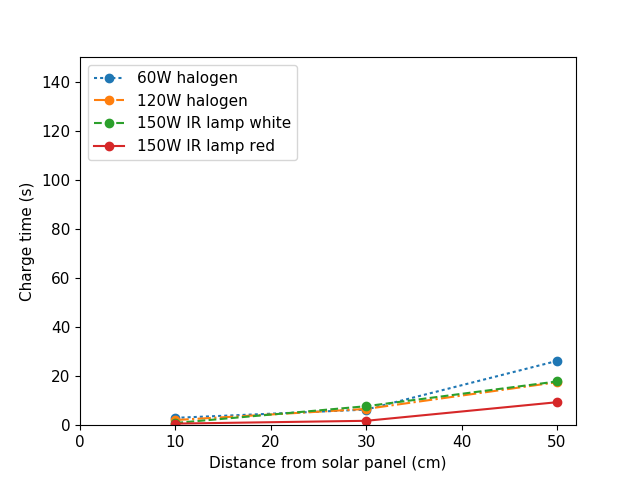
\includegraphics[width=\textwidth]{pics/light_experiment_figure1.png}
		\caption{Ebay panel}
		\label{fig:light_exp1}
	\end{subfigure}
	\begin{subfigure}[b]{0.49\textwidth}
		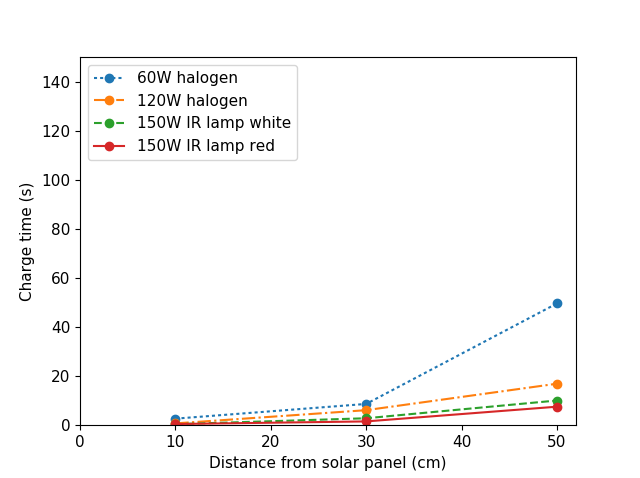
\includegraphics[width=\textwidth]{pics/light_experiment_figure2.png}
		\caption{IXYS SLMD121H04L-ND}
		\label{fig:light_exp2}
	\end{subfigure}
	\begin{subfigure}[b]{0.49\textwidth}
		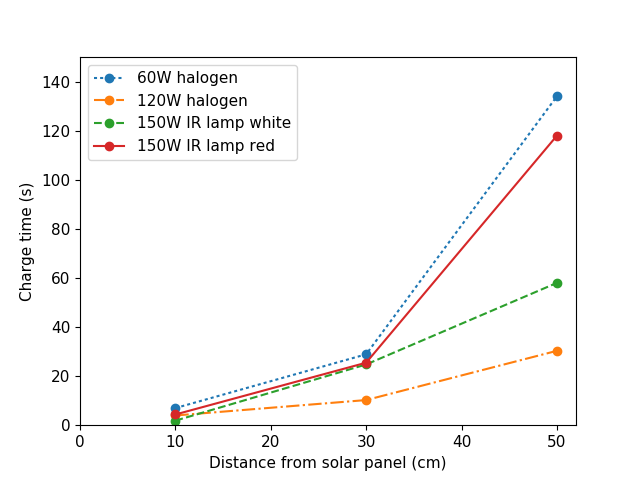
\includegraphics[width=\textwidth]{pics/light_experiment_figure3.png}
		\caption{Azurspace 3G28C}
		\label{fig:light_exp3}
	\end{subfigure}
	\caption{The performance of three different solar panels for different distances from different light sources. The data charge times for the last two are normalized with respect to the surface covered by the first panel.}
\end{figure}

\section{Controlled movements}

Now that the best performing solar panel / light combination has been found, a performance comparison can be made between the battery-less robot and it's battery powered equal.

\subsection{Experimental setup}

\section{Results}

% Comparison deadreckoning accuracy of battery powered robot with solar powered robot

% Try at least one more supercapacitor: 10mF
% Study reducing the frequency of power interrupts ie smaller energy buffer.
% How does this effect the accuracy of locomotion?

% Study the effect of checkpoint frequency on the straight and turn accuracy + combination
% Before and after counting in case of current robot

% Video of robot movement

